\documentclass{VUMIFPSkursinis}
\usepackage{algorithmicx}
\usepackage{algorithm}
\usepackage{algpseudocode}
\usepackage{amsfonts}
\usepackage{amsmath}
\usepackage{bm}
\usepackage{caption}
\usepackage{color}
\usepackage{float}
\usepackage{graphicx}
\usepackage{listings}
\usepackage{subfig}
\usepackage{wrapfig}

% Titulinio aprašas
\university{Vilniaus universitetas}
\faculty{Matematikos ir informatikos fakultetas}
\department{Programų sistemų katedra}
\papertype{Programų kūrimo proceso laboratorinis darbas}
\title{Įmonės ,,Mėnuliukai technologies" programų kūrimo proceso aprašas (Pirmas laboratorinis darbas)}
\titleineng{Description of the development process of the ,,Moon technologies" company ("First laboratory work")}
\status{4 kurso 3 grupės studentai}
\author{Matas Savickis, Justas Tvarijonas, Džiugas Mažulis}
\secondauthor{Greta Pyrantaitė, Andrius Bentkus}


\supervisor{Saulius Ragaišis, Doc., Dr.}
\date{Vilnius – \the\year}

% Nustatymai
% \setmainfont{Palemonas}   % Pakeisti teksto šriftą į Palemonas (turi būti įdiegtas sistemoje)
\bibliography{bibliografija}

\begin{document}
\maketitle

\tableofcontents

\sectionnonum{Įvadas}
Šiame darbe bus pristatyta ,,Mėnuliukai techynologies" programų kūrimo procesas. Pats procesas yra paremtas Agile metodologija su minimaliais pakeitimai reikalavimų rinkime. Tikimės, kad kūrimo procesas bus labiau pritaikytas dirbti su projektais, kurių pradžioje reikalinga surinkti daugiau informacijos ir tūrėti aiškesnį kryptį, kas bus toliau. Procesas gali vykti dviem būdais:
\begin{itemize}
	\item{Klientas perka sistemą, kuri turės atitinkamus funkcionalumus - projekto pradžioje yra išsiaiškinama koks funkcionalumas turi būti sistemoje}
	\item{Klientas perka sistemos tobulinimo valandas - projekto pradžioje klientas pateikia funkcionalumų, kuriuos jis nori tūrėti sąrašą prioriteto tvarka. Klientas nusiperka tam tikrą skaičių darbo valandų ir tuomet laikui bėgant programuotų komanda įvertina kiek užtruks tam tikro funkcionalumo įgyvendinimas. Pasibaigus nusipirktom valandom nauji pakeitimai nebetiekiami kol klientas nenusiperka papildomų darbo valandų.}
\end{itemize}
\section{Kūrimo procesas}

	\begin{figure}[H]
	\centering
	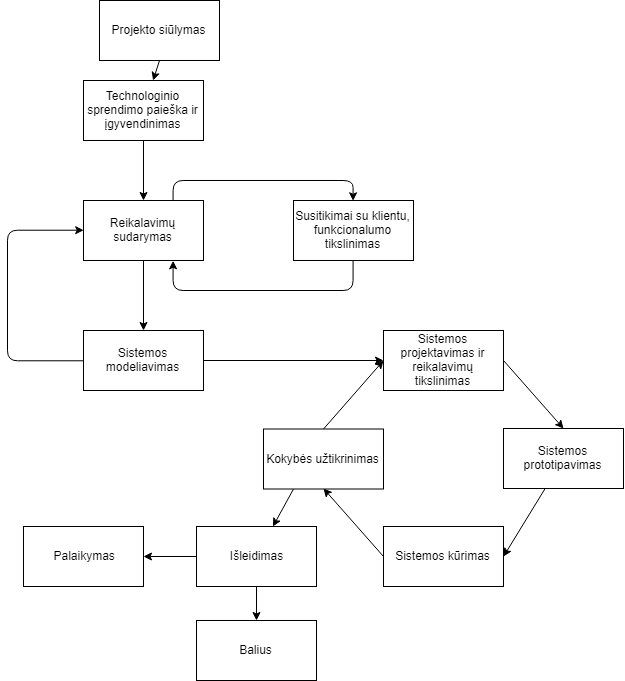
\includegraphics[scale=0.7]{img/SoftwareProcessMoonTechnologies}
	\caption{Sistemos kūrimo procesas} % Antraštė įterpiama po paveikslėlio
	\label{img:mlp}
	\end{figure}

	\subsection{Projekto siūlymas}
		Tai yra pradinė projekto fazė, kurioje yra užmezgamas dialogas su klientų. Per viešuosius pirkimus arba pačiam klientui susisiekus su įmone prasideda abstrakti sistemos analizė ir pasiūlymo sudarymas. Abstrakčioje sistemos analizėje įvertinami pagrindiniai kliento poreikei, buvusių projektų patirtis, projekto kompleksiškumas ir dabartinė įmonės būsena. Įvertinama ar įmonė turi visus reikiamus specialistus atlikti darbui, kiek žmonių jau yra įmonėje, kiek reiktų pasisamdyti arba kokius dabus perduoti sub-kontraktoriams.

	\subsection{Technologinio sprendimo paieška ir įgyvendinimas}
		Pasirašius sutartį su klientu pradedama ieškoti konkretaus technologinio sprendimo tinkako projekto vystimui. Sutatomos konrečios karkasų, duomenų bazių arba betkokios kitos technologijos versijos kurios bus naudojamos. Jeigu projektas yra jau egzistuojantis ir klientas perka tolimesnį projekto vystimą yra išsiaiškinama ar dėl saugumo priežasčių nereikės pakelti projekte naudojamų technologijų versijos.
	\subsection{Reikalavimų ciklas}
		Nutarus dėl konkrečių technologijų kurios bus naudojamos pradedame funkcinių ir nefunkcinių reikalavimų sudarymas. Jų sudarymas vyksta cikliškai, pirma mūsų įmonės verslo analitikas išanalizuoja verslo poreikius ir kartu su architektu sudaro pirminius reikalavimus, jie yra pristatomi klientui kartu su klausimais, įvyksta suformuotų reikalavimų aptarimas. Jeigu klientas sutinka su sudarytais reikalavimais pradedamas sistemos maketavimas, jeigu kyla neaiškumų dėl reikalavimų tarp kliento ir mūsų įmonės grįštama prie poreikių sudarimo įmonės viduje. Ciklas vyksta iki tol kol pasiekiamas sutarimas tarp mūsų įmonės ir kliento.
	\subsection{Sistemos maketas}
	\subsection{Sistemos projektavimas}
	\subsection{Sistemos prototipavimas}
	\subsection{Sistemos kūrimas}
	\subsection{Kokybės užtikrinimas}
	\subsection{Išleidimas}
	\subsection{Palaikymas}
	\subsection{Balius/Post-mortem}
	



\sectionnonum{Rezultatai ir išvados}




\end{document}
